% ---------------------------------------------------------------------------
% ---------------------------------------------------------------------------
% Modelo LaTex para preparação do documento final de Monografia TCC
% O modelo em conformidade com ABNT NBR
% IMT
% ---------------------------------------------------------------------------
% ---------------------------------------------------------------------------

\documentclass[
	% -- opções da classe memoir --
	12pt,					% tamanho da fonte
	openright,				% capítulos começam em pág ímpar (insere página vazia caso preciso)
	oneside,					% para impressão em verso e anverso. Oposto a oneside
	a4paper,					% tamanho do papel. 
	% -- opções da classe abntex2 --
	%chapter=TITLE,			% títulos de capítulos convertidos em letras maiúsculas
	%section=TITLE,			% títulos de seções convertidos em letras maiúsculas
	%subsection=TITLE,		% títulos de subseções convertidos em letras maiúsculas
	%subsubsection=TITLE,	% títulos de subsubseções convertidos em letras maiúsculas
	% -- opções do pacote babel --
	english,					% idioma adicional para hifenização
	%french,					% idioma adicional para hifenização
	%spanish,				% idioma adicional para hifenização
	brazil					% o último idioma é o principal do documento
	]{abntex2}

% ---------------------
% Pacotes OBRIGATÓRIOS
% ---------------------
\usepackage{mathptmx}				% Usa a fonte Latin Modern			
\usepackage[T1]{fontenc}			% Selecao de codigos de fonte.

\renewcommand{\ABNTEXchapterfont}{\fontfamily{ptm}\selectfont}
\renewcommand{\ABNTEXpartfont}{\fontfamily{ptm}\selectfont}
\renewcommand{\ABNTEXsectionfont}{\fontfamily{ptm}\selectfont}
\renewcommand{\ABNTEXsubsectionfont}{\fontfamily{ptm}\selectfont}
\renewcommand{\ABNTEXsubsubsectionfont}{\fontfamily{ptm}\selectfont}

\usepackage[utf8]{inputenc}		% Codificacao do documento (conversão automática dos acentos)
\usepackage{lastpage}			% Usado pela Ficha catalográfica
\usepackage{indentfirst}		% Indenta o primeiro parágrafo de cada seção.
\usepackage{color}				% Controle das cores
\usepackage{graphicx,graphicx}	% Inclusão de gráficos
\usepackage{epsfig,subfig}		% Inclusão de figuras
\usepackage{microtype} 			% Melhorias de justificação
% ---------------------
		
% ---------------------
% Pacotes ADICIONAIS
% ---------------------
\usepackage{multirow}
\usepackage{lipsum}						% Geração de dummy text
\usepackage{amsmath,amssymb,mathrsfs}	% Comandos matemáticos avançados 
\usepackage{setspace}  					% Para permitir espaçamento simples, 1 1/2 e duplo
\usepackage{verbatim}					% Para poder usar o ambiente "comment"
\usepackage{tabularx} 					% Para poder ter tabelas com colunas de largura auto-ajustável
\usepackage{afterpage} 					% Para executar um comando depois do fim da página corrente
\usepackage{url}
\usepackage{gensymb}
% Para formatar URLs (endereços da Web)
% --- Adicionados para este trabalho ---
\usepackage{booktabs}					% tabelas com filetes (\toprule etc.)
\usepackage{xcolor}
\AtBeginDocument{\renewcommand{\ohm}{\ensuremath{\Omega}}} % glifo do gensymb some com mathptmx
% Pendência visível no PDF (remover antes da entrega)
\newcommand{\pendente}[1]{\textcolor{red}{\textbf{[PENDENTE: #1]}}}
% Figuras internas do projeto.
\graphicspath{{images/}{figures/}}
% ---------------------

% ---------------------
% Pacotes de CITAÇÕES
% ---------------------
%\usepackage[brazilian,hyperpageref]{backref}	% Paginas com as citações na bibl
\usepackage[alf]{abntex2cite}				% Citações padrão ABNT (alfa)

%\usepackage[num]{abntex2cite}				% Citações padrão ABNT (numericas)
% ---------------------
\usepackage{float}
% Configurações de CITAÇÕES para abntex2
%% --- 
% CONFIGURAÇÕES DE PACOTES
% --- 

% ---
% Configurações do pacote backref
% Usado sem a opção hyperpageref de backref
%\renewcommand{\backrefpagesname}{Citado na(s) página(s):~}
% Texto padrão antes do número das páginas
%\renewcommand{\backref}{}
% Define os textos da citação
%\renewcommand*{\backrefalt}[4]{
%	\ifcase #1 %
%		Nenhuma citação no texto.%
%	\or
%		Citado na página #2.%
%	\else
%		Citado #1 vezes nas páginas #2.%
%	\fi}%
% ---

% Inclui Configurações de aparência do PDF Final
%  Configurações de aparência do PDF final
% NÃO ALTERAR!!!

% alterando o aspecto da cor azul
\definecolor{blue}{RGB}{41,5,195}

% informações do PDF
\makeatletter
\hypersetup{
     	%pagebackref=true,
		pdftitle={\@title}, 
		pdfauthor={\@author},
    		pdfsubject={\imprimirpreambulo},
	    pdfcreator={LaTeX with abnTeX2},
		pdfkeywords={abnt}{latex}{abntex}{abntex2}{trabalho acadêmico}, 
		colorlinks=true,       		% false: boxed links; true: colored links
    		linkcolor=black,          	% color of internal links
    		citecolor=black,        		% color of links to bibliography
    		filecolor=magenta,      		% color of file links
		urlcolor=black,
		bookmarksdepth=4
} 
\makeatother
% --- 
\hypersetup{hypertexnames=false} % destinos unicos, mesmo com a contagem reiniciada na capa

% O tamanho da identação do parágrafo é dado por:
\setlength{\parindent}{0cm}
\setlength{\parskip}{0.2cm} 
% Controle do espaçamento entre um parágrafo e outro:
\setlength{\parskip}{0.2cm}  % tente também \onelineskip

% Ajusta o espaçamento após \chapter
\setlength\afterchapskip{\lineskip}

\setlist[itemize]{leftmargin=1.25cm}
\setlist[enumerate]{leftmargin=1.25cm}
\usepackage{listings}
\usepackage{framed}
% ---------------------
% Compila o indice
% ---------------------
\makeindex
% ---------------------

%%%%%%%%%%%%%%%%%%%%%%%%%%%
%%  INICIO DO DOCUMENTO  %%
%%%%%%%%%%%%%%%%%%%%%%%%%%%
\begin{document}

% Retira espaço extra obsoleto entre as frases.
\frenchspacing

% ----------------------------------------------------------
% ELEMENTOS PRÉ-TEXTUAIS (Capa, Resumo, Abstract, etc.)
% ----------------------------------------------------------
\pretextual

% Elementos textuais com numeração arábica
\pagenumbering{arabic}

% Capa
% ---
% Impressão da Capa
% ---
  \begin{capa}%
    \center
    
\includegraphics[scale=0.12]{images/logo_IMT_preto_1.png} \\
	{\fontfamily{ptm}\selectfont
        \ABNTEXchapterfont\large{CENTRO UNIVERSITÁRIO DO INSTITUTO MAUÁ DE TECNOLOGIA \\
                                        Engenharia de Controle e Automação}
    }
	
    \vspace{1cm}
    {\fontfamily{ptm}\selectfont
        \LARGE{Sistemas Inteligentes Aplicados à Ergonomia no Ambiente de Trabalho}
    }
    \vspace{1cm}
    
    %%%%%%%%%%%%%%%%% INFORMAÇÕES SOBRE AUTOR PRINCIPAL %%%%%%%%%%%%%%%%%%%%%%%%%%%%%%%
    {\fontfamily{ptm}\selectfont
        \begin{flushright}
            \normalsize{André Thomas Monteiro} \\
            \normalsize{Felipe Fernandes Rojas Godoi} \\
            \normalsize{Vinicius Carnicelli Beleti} \\
            \normalsize{Orientadora: Profa. Me. Andressa Corrente Martins} \\
        \end{flushright}
    }
    \vspace{0.2cm}

    %%%%%%%%%%%%%%%%%%%%%%%%%%%%%%%% RESUMO %%%%%%%%%%%%%%%%%%%%%%%%%%%%%%%
    
    \setlength{\absparsep}{18pt} % ajusta o espaçamento dos parágrafos do resumo
    \begin{abstract}
        \noindent
        % Resumo: parágrafo único, no máximo 1160 caracteres (modelo IMT).
Os distúrbios osteomusculares atingem a maioria dos trabalhadores de escritório e estão associados a posturas inadequadas prolongadas. Este trabalho desenvolve um sistema embarcado que detecta postura sentada prejudicial e alerta o usuário por vibração. Uma cadeira com oito sensores de força resistivos mede a distribuição do peso; um colar com sensor inercial mede a orientação da parte superior das costas. O sistema, calibrado pela postura ereta de cada usuário, funde as duas fontes e envia o alerta ao colar por rádio. Em testes com oito participantes, cada um avaliado fora do ajuste, o sistema alertou em 94\,\% dos trechos de postura prejudicial, com alerta em 3\,\% do tempo em postura ereta ou reclinada. A fusão eliminou a maior parte dos falsos alarmes ao reclinar e passou a detectar o escorregamento do quadril. Os resultados indicam a viabilidade técnica da abordagem; a projeção isolada da cabeça permanece como principal limitação.

\vspace{0.2cm}

\textbf{Palavras-chave:} Monitoramento postural. Fusão de sensores.

    \end{abstract}

\end{capa}
% ---
\clearpage

% Resumo e Abstract
% ---
% RESUMOS
% ---

\setlength{\absparsep}{18pt} % ajusta o espaçamento dos parágrafos do resumo
\selectlanguage{english}

\begin{abstract}
    \noindent
    Musculoskeletal disorders affect most office workers and are associated with poor postures held for long periods. This work develops an embedded system that detects harmful sitting posture and alerts the user through vibration. A chair with eight force-sensing resistors measures how body weight is distributed, and a collar with an inertial sensor measures the orientation of the upper back. The chair fuses both sources, calibrated to each user's upright posture, and sends the alert to the collar over radio. In tests, each evaluated outside parameter tuning, the system alerted in 94\,\% of harmful-posture segments, while alerting during 3\,\% of upright or reclined time. Fusion removed most false alarms when reclining and enabled the detection of the hips sliding forward. The results indicate the technical feasibility of the approach; isolated head protraction remains the main limitation.

\vspace{0.2cm}

\textbf{Keywords:} Posture monitoring. Sensor fusion.


\end{abstract}

\clearpage

% ----------------------------------------------------------
% ELEMENTOS TEXTUAIS (Capítulos)
% ----------------------------------------------------------
\textual

% Reinicia a contagem do número de páginas
\setcounter{page}{3}

% Inclui cada capitulo da Dissertação
\begingroup
    \selectlanguage{brazil}
    \renewcommand{\fontename}{Fonte} % o abstract em inglês deixa "Source"

    \renewcommand{\cleardoublepage}{}
    \renewcommand{\clearpage}{}
    
    \chapter{Introdução}\label{cap:introducao}

O trabalho em escritório, presencial ou remoto, impõe longas jornadas
sentadas, e os distúrbios osteomusculares relacionados ao trabalho (DORT)
atingem entre 71,9\,\% e 80,81\,\% dos trabalhadores de escritório,
sobretudo no pescoço, nos ombros e na coluna lombar
\cite{okezue2020,mohammadian2025}. Como manter a postura correta depende da
atenção contínua do trabalhador, um aviso no momento em que ela se degrada
pode torná-la hábito sem supervisão.

Define-se, assim, o problema de pesquisa: \emph{como um sistema embarcado de
baixo custo pode detectar, em tempo real, posturas sentadas prejudiciais e
avisar o usuário para que ele se corrija?} Dois fatores dificultam a
detecção: a ``postura correta'' varia de pessoa para pessoa, e um único tipo
de sensor não distingue situações, reclinar no encosto
(aceitável) e escorregar o quadril para a frente (prejudicial) inclinam o
tronco no mesmo sentido.

A proposta combina a distribuição do peso sobre a cadeira, medida por
sensores de força no assento e no encosto, com a orientação da parte superior
das costas, medida por uma unidade de medição inercial (IMU) em um colar; o sistema funde as duas informações e, se a postura for prejudicial por tempo
suficiente, o colar vibra. Justifica-se o trabalho pelo monitoramento
individual e contínuo com componentes acessíveis, sem câmeras, aplicativo ou
nuvem.

\section{Objetivos}

O objetivo geral é desenvolver um sistema embarcado, composto por uma
cadeira de escritório instrumentada e um colar com sensor inercial, capaz de
detectar posturas sentadas prejudiciais e alertar o usuário em tempo real por
vibração. Os objetivos específicos são:

\begin{itemize}
  \setlength{\itemsep}{0pt}
  \setlength{\parsep}{0pt}
  \item Caracterizar a variação da postura de referência entre
        usuários e entre colocações do sensor, e propor uma calibração
        individual que a compense;
  \item Construir e integrar o colar e a cadeira instrumentada,
        com comunicação sem fio entre eles;
  \item Implementar o alerta ao usuário por vibração, com
        sinalização de estado;
  \item Avaliar a capacidade de detecção do sistema com
        múltiplos participantes.
\end{itemize}


    \renewcommand{\cleardoublepage}{}
    \renewcommand{\clearpage}{}
    
    \chapter{Revisão Bibliográfica}\label{cap:fund_teorica}

Este capítulo reúne os fundamentos que orientam o projeto: os critérios de
avaliação do risco da postura sentada, as características dos sensores de
força e inerciais usados para medi-la e os trabalhos que monitoram a postura
na cadeira ou no corpo, com ou sem retorno ao usuário. Ao final, identifica-se
a lacuna que o sistema proposto procura ocupar.

\section{Postura sentada e avaliação postural}
\label{sec:rev-ergonomia}

Os DORT afetam músculos, tendões, articulações e nervos. Entre seus fatores de
risco estão a postura inadequada, a permanência prolongada em posição estática
e a ausência de pausas, agravados por fatores psicossociais
\cite{mohammadian2025}. O risco postural costuma ser avaliado por métodos
observacionais: o RULA \cite{mcatamney1993} pontua faixas de ângulo de
inclinação do tronco e do pescoço, o pescoço é penalizado em faixas de
10\degree{} de flexão, e a norma ISO 11226 \cite{iso11226} combina o ângulo
com o tempo de manutenção da postura. Ângulo do tronco e persistência
no tempo fundamentam, neste trabalho, a inclinação medida por IMU e a espera
antes do alerta; os limiares do sistema, porém, são desvios em relação à
postura de referência de cada usuário, e não ângulos absolutos de norma.

\section{Sensores para monitoramento postural}
\label{sec:rev-sensores}

O FSR (\emph{Force Sensing Resistor}) é um filme polimérico cuja resistência cai à medida que a força aplicada aumenta. O FSR402 tem área ativa
de 12{,}7\,mm de diâmetro, faixa de cerca de 0{,}2 a 20\,N, curva
força--resistência fortemente não linear, repetibilidade de $\pm$6\,\% entre
peças e deriva sob carga constante (\emph{creep}) inferior a 5\,\% por década
de tempo \cite{interlink_datasheet}. O \emph{creep}, de origem viscoelástica, é
a limitação mais relevante para quem permanece sentado por longos períodos
\cite{paredesmadrid2017}, e o fabricante adverte que o FSR não é uma célula de
carga: a exatidão em força varia de $\pm$6\,\% a $\pm$50\,\% conforme a
montagem \cite{interlink_guia}. O FSR serve, portanto, como medida
\textbf{relativa} de distribuição de carga, comparando sensores entre si ou com
uma linha de base própria.

\textbf{Acelerômetros e IMUs.} Em repouso, o acelerômetro mede o vetor
gravidade no referencial do sensor, do qual se obtêm os ângulos de arfagem
(\emph{pitch}) e rolagem (\emph{roll}). A estimativa supõe aceleração linear
desprezível, não observa a guinada (\emph{yaw}) e é instável perto de
$\pm$90\degree{} de arfagem \cite{pedley2013}; movimentos dinâmicos exigem
combiná-lo ao giroscópio. Como a postura sentada é quase estática, este
trabalho usa apenas o acelerômetro. O ângulo absoluto, porém, depende de como
o sensor assenta nas costas a cada uso, o que motiva a calibração por usuário.

\section{Trabalhos relacionados}
\label{sec:rev-relacionados}

As primeiras cadeiras instrumentadas usavam mapas de pressão de alta
resolução \cite{tan2001}; as seguintes passaram a poucos sensores discretos.
\citeonline{zemp2016} combinaram 16 FSRs a um módulo inercial no encosto, que
mede a inclinação da cadeira, e não a do usuário, e classificaram sete
posições. Nesses trabalhos a saída é a classificação da postura, sem retorno ao
usuário. O LifeChair, almofada com sensores de pressão, vibração e aplicativo,
acrescenta o retorno e observa que o índice de massa corporal altera o padrão
de pressão \cite{bourahmoune2019}. Do lado vestível, um sensor no tronco que
vibra quando este se curva reduziu a flexão do pescoço e a cifose torácica de
21 adultos durante uma hora de digitação \cite{kuo2021}. A vibração não ocupa
a visão, já dedicada à tela, mas é percebida como o retorno mais intrusivo
\cite{haller2011}, e a evidência de efeito sustentado é fraca: em ensaio com
trabalhadores, o retorno sobre a postura lombar não diferiu do grupo controle
\cite{ribeiro2014}. O alerta deve, assim, disparar só depois que o desvio
persiste, e o efeito em longo prazo não pode ser presumido a partir de testes
curtos.

Na revisão sistemática de \citeonline{kappattanavar2021}, 13 dos 14
estudos usavam sensores de pressão e nenhum os combinava a um IMU no corpo.
O sistema proposto ocupa essa lacuna em quatro aspectos: funde a
distribuição de peso na cadeira com a orientação do tronco superior, que não
toca a cadeira, de modo que cada canal cobre casos que o outro confunde
(reclinar inclina o tronco sem ser prejudicial; escorregar descarrega o apoio
traseiro do assento com pouca inclinação); fornece retorno háptico em
tempo real no corpo; usa calibração por usuário, em vez de limiares
absolutos ou modelos treinados em outras pessoas; e faz todo o
processamento embarcado, sem aplicativo nem nuvem.


    \renewcommand{\cleardoublepage}{}
    \renewcommand{\clearpage}{}
    
    \chapter{Metodologia}\label{cap:metodologia}

O sistema combina as informações obtidas pelo colar no alto da coluna, com as obtidas pelos oito sensores de força na cadeira para alertar o usuário que estiver em postura incorreta. 

\begin{figure}[H]
    \centering
    \caption{Fotografia do sistema.}
    \begin{minipage}{0.48\textwidth}
        \centering
        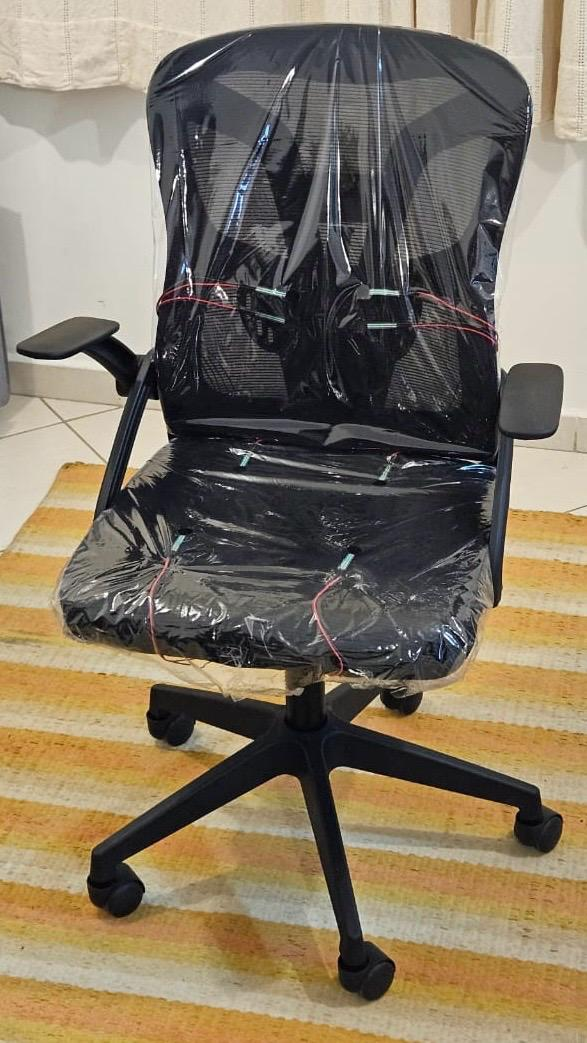
\includegraphics[width=\linewidth,height=260.3469pt]{WhatsApp Image 2026-11-15 at 11.15.11.jpeg}
    \end{minipage}
    \hfill
    \begin{minipage}{0.48\textwidth}
        \centering
        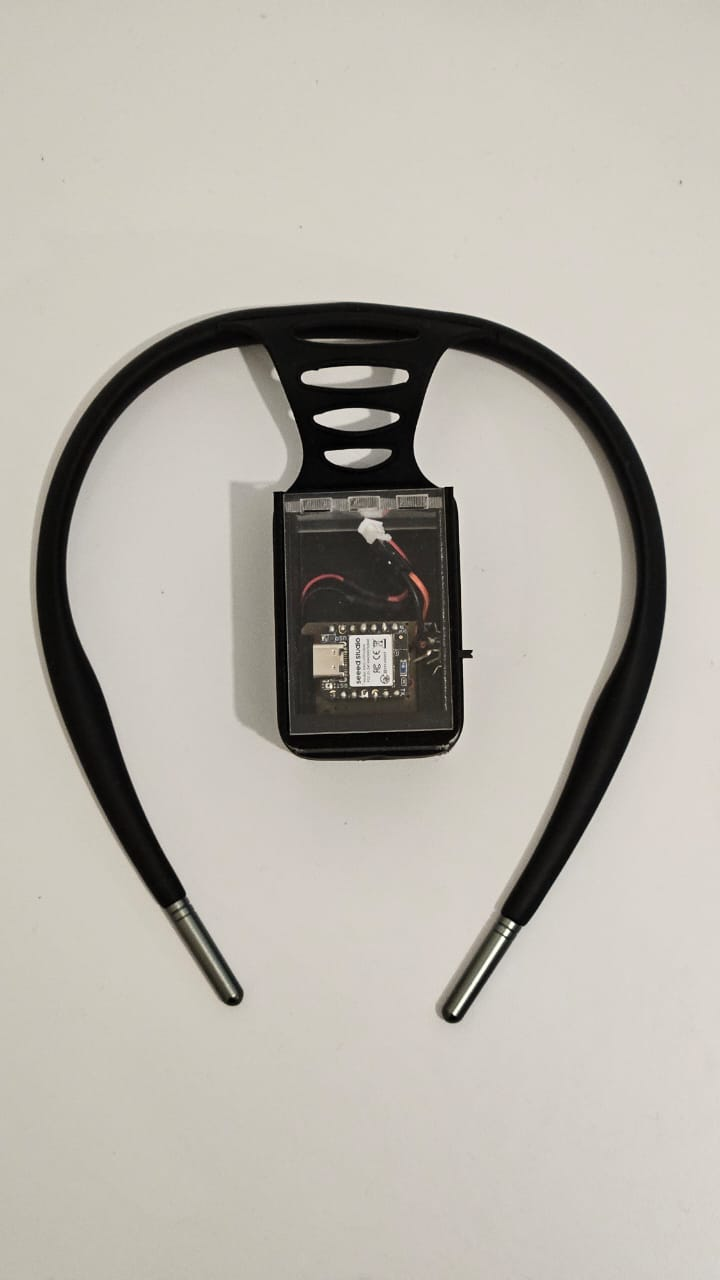
\includegraphics[width=\linewidth,height=260.3469pt]{Colar (solo).jpeg}
    \end{minipage}

    \fonte{Fotografado pelos autores (2026)}
    \label{fig:sistema}
\end{figure}

\section{Colar}
\label{sec:met-colar}

O colar contém uma placa XIAO nRF52840 Sense com IMU LSM6DS3TR-C
\cite{seeed_xiao,nordic_nrf52840,st_lsm6ds3trc}, posicionada nas costas,
abaixo do pescoço, como mostra a Figura~\ref{fig:met-foto-colar}.

\begin{figure}[H]
 \centering
 \caption{Fotografia da posição do colar.}
 \begin{SingleSpace}
 \raisebox{-0.0pt}{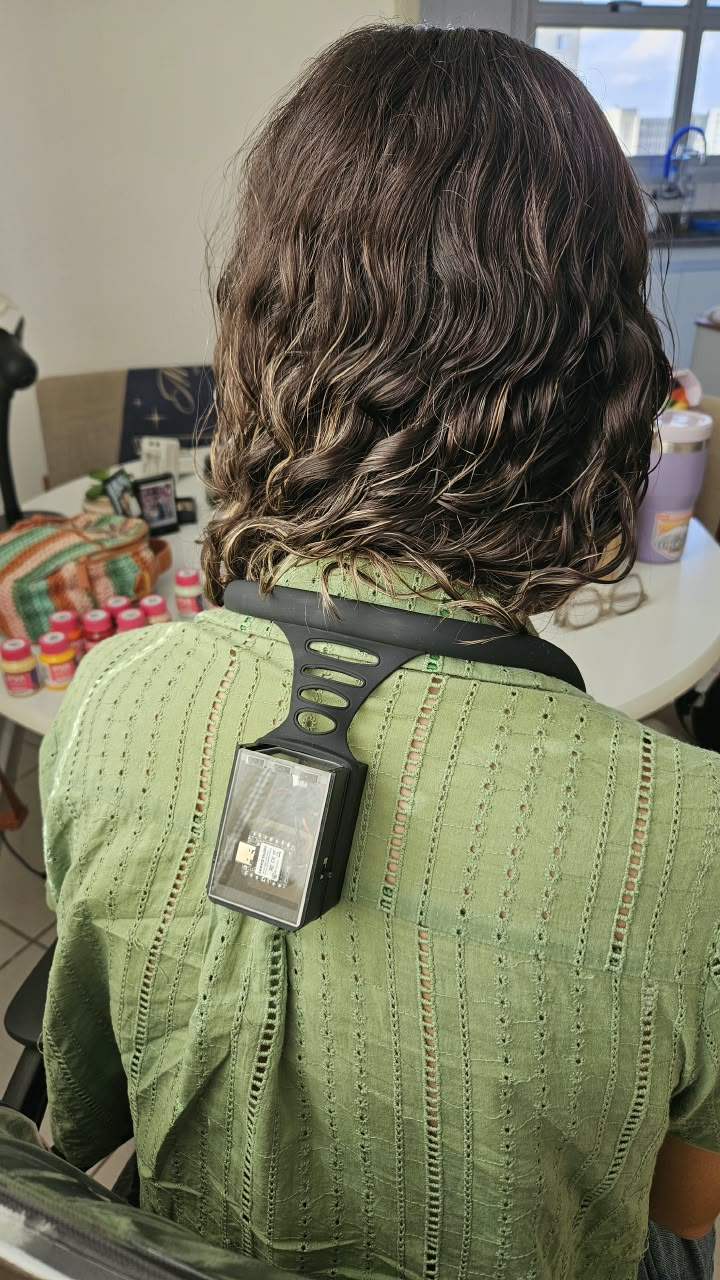
\includegraphics[width=190pt,height=260.3469pt]{Colar (pescoço).jpeg}}
 \end{SingleSpace}
 \fonte{Fotografado pelos autores (2026)}
 \label{fig:met-foto-colar}
\end{figure}

Mede-se a orientação local, não a curvatura de toda a
coluna. Utiliza-se apenas o acelerômetro, com giroscópio desligado.
Das componentes $a_x$, $a_y$ e $a_z$, calculam-se \textit{pitch} ($p$)
e \textit{roll} ($r$), em graus:
\begin{equation}
 p=\frac{180}{\pi}\operatorname{atan2}\!\left(-a_x,\sqrt{a_y^2+a_z^2}\right),
 \qquad r=\frac{180}{\pi}\operatorname{atan2}(a_y,a_z).
 \label{eq:met-angulos}
\end{equation}
A estimativa usa a gravidade em condição aproximadamente estática
\cite{pedley2013}. Na montagem, $p$ é lateral (positivo à direita) e $r$,
sagital (negativo para a frente). Adquire-se e transmite-se a 20\,Hz;
movimento, deslocamento do colar e vibração podem alterar a medida.
Leituras inválidas inibem o alerta.

No circuito da Figura~\ref{fig:met-esquema-colar}, o transistor BC337
aciona o motor por modulação por largura de pulso (PWM), pois sua corrente
excede a de um pino lógico.
O diodo protege o chaveamento e o capacitor atenua o ruído. Durante os
pulsos de 700\,ms, separados por 300\,ms, transmite-se a última orientação
sem vibração, por até 1{,}5\,s. A Figura~\ref{fig:met-fluxo-colar}
sintetiza a aquisição e o controle.

\begin{figure}[H]
 \centering
 \caption{Esquema elétrico do colar.}
 \begin{SingleSpace}
 \raisebox{-0.0pt}{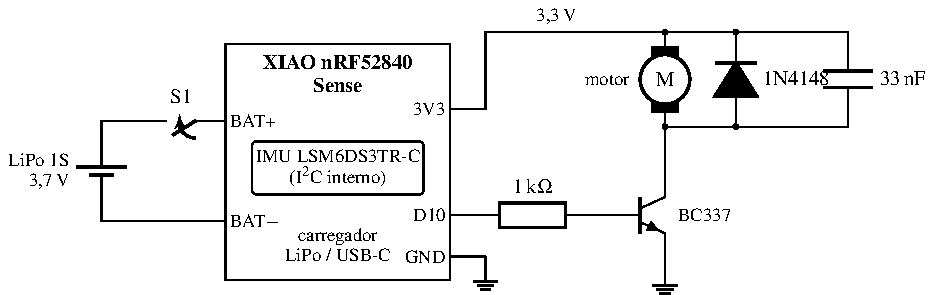
\includegraphics[width=448.00436pt,height=142.3469pt]{met-esquema-colar.pdf}}
 \end{SingleSpace}
 \fonte{Elaborado pelos autores (2026)}
 \label{fig:met-esquema-colar}
\end{figure}

\begin{figure}[H]
 \centering
 \caption{Fluxo de aquisição, controle e proteção do colar.}
 \begin{SingleSpace}
 \raisebox{-0.0pt}{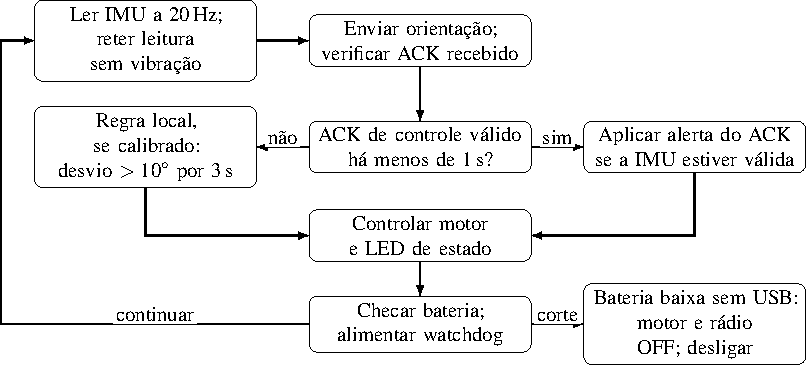
\includegraphics[width=388.42339pt,height=175.91806pt]{met-fluxo-colar.pdf}}
 \end{SingleSpace}
 \fonte{Elaborado pelos autores (2026)}
 \label{fig:met-fluxo-colar}
\end{figure}

A alimentação usa LiPo 1S de 3{,}7\,V, chave S1 e recarga pelo USB-C
do XIAO; o invólucro comporta 1800\,mAh. Sem USB, três leituras abaixo de
3{,}30\,V desligam o colar; a partida exige 3{,}40\,V. O LED sinaliza
enlace, calibração, alerta e falha.

\section{Cadeira}
\label{sec:met-cadeira}

A segunda placa XIAO lê oito FSR402: quatro no assento (frente/trás,
esquerda/direita) e quatro no encosto (superior/inferior, esquerda/direita).
Sua resistência diminui com a força \cite{interlink_datasheet}; usam-se
as leituras como contato e distribuição relativa, sem conversão em força
absoluta na espuma.

O circuito da Figura~\ref{fig:met-esquema-cadeira} usa o multiplexador
CD74HC4067 \cite{ti_cd74hc4067} para ligar cada FSR ao resistor
compartilhado de 3{,}3\,k\ohm{} em SIG. Incluindo a resistência de
condução $R_{\mathrm{on}}$, a tensão lida em A0 é
\begin{equation}
 V_{\mathrm{SIG}}=V_{\mathrm{DD}}
 \frac{R_{\mathrm{fixo}}}{R_{\mathrm{fixo}}+R_{\mathrm{FSR}}+R_{\mathrm{on}}}.
 \label{eq:met-divisor}
\end{equation}
A tensão aumenta com a carga. O resistor aproxima
$\sqrt{R_{\min}R_{\max}}$ na faixa de contato, como compromisso entre
resolução e corrente; o efeito fixo de $R_{\mathrm{on}}$ é incorporado à
calibração. Os oito canais são lidos a 20\,Hz, com ADC de 12 bits.
O botão D9 solicita a calibração. A alimentação repete o circuito do colar.

\begin{figure}[H]
 \centering
 \caption{Esquema elétrico da cadeira.}
 \begin{SingleSpace}
 \raisebox{-0.0pt}{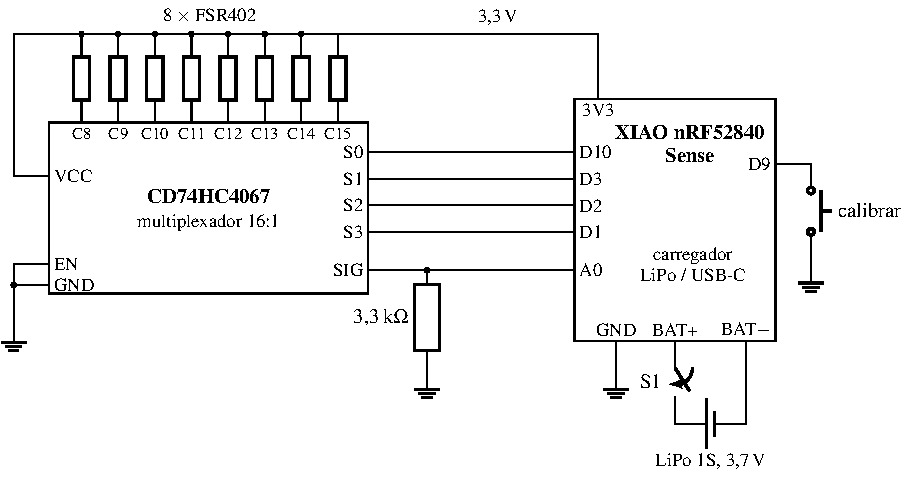
\includegraphics[width=436.23093pt,height=230.01868pt]{met-esquema-cadeira.pdf}}
 \end{SingleSpace}
 \fonte{Elaborado pelos autores (2026)}
 \label{fig:met-esquema-cadeira}
\end{figure}

\section{Integração}
\label{sec:met-integracao}

A Figura~\ref{fig:met-arquitetura} reúne os blocos. O enlace Nordic
Enhanced ShockBurst (ESB), pela biblioteca \texttt{nrf\_to\_nrf}, usa
confirmação (ACK) e retransmissão
\cite{nordic_esb,tmrh20_nrftonrf}. A decisão da amostra $N$ retorna no ACK
de $N+1$. Após 1\,s sem ACK válido, o colar aplica a regra inercial
à última referência recebida; sem referência, não alerta.

\begin{figure}[H]
 \centering
 \caption{Arquitetura autônoma e interfaces de acompanhamento.}
 \begin{SingleSpace}
 \raisebox{-0.0pt}{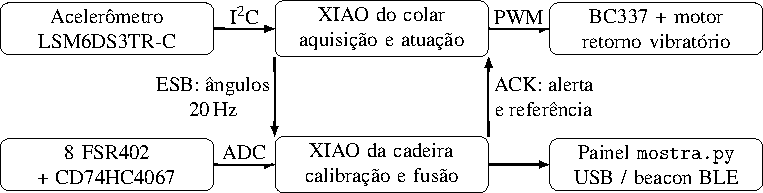
\includegraphics[width=367.74976pt,height=92.78621pt]{met-arquitetura.pdf}}
 \end{SingleSpace}
 \fonte{Elaborado pelos autores (2026)}
 \label{fig:met-arquitetura}
\end{figure}

A calibração individual é acionada com o usuário ereto, sentado ao fundo.
Em 20 amostras válidas (cerca de 1\,s), capturam-se as médias angulares
$p_0$, $r_0$ e a linha de base $b_i$ de cada FSR. Recusa-se a captura com
falha de IMU/enlace ou base traseira $B_T=b_{TE}+b_{TD}<1000$ contagens.
A referência é volátil e deve ser refeita após reinício ou recolocação.

Na fusão, $FE$, $FD$, $TE$ e $TD$ indicam frente/trás e esquerda/direita do
assento. O encosto é registrado e exibido, mas não decide o alerta, pois
pode ficar sem carga mesmo no ereto. Para leituras $f_i$, definem-se
\begin{equation}
 \begin{gathered}
 \Delta p=p-p_0,\quad \Delta r=r-r_0,\quad
 d=\sqrt{\Delta p^2+\Delta r^2},\\
 S=f_{FE}+f_{FD}+f_{TE}+f_{TD},\qquad
 \rho=\frac{f_{TE}+f_{TD}}{B_T},\\
 \ell=\frac{f_{FE}+f_{TE}-f_{FD}-f_{TD}}{S}
      -\frac{b_{FE}+b_{TE}-b_{FD}-b_{TD}}{\sum_{i\in\mathrm{assento}}b_i}.
 \end{gathered}
 \label{eq:met-indicadores}
\end{equation}
A razão $\rho$ mede o apoio traseiro relativo à referência; $\ell$, a
redistribuição lateral, positiva à esquerda. Para confirmar inclinação,
$h=\ell$ se $\Delta p<0$, ou $h=-\ell$ caso contrário; exige-se base
total do assento $\geq2000$ contagens. O teste de vazio precede as divisões.
Com $\Delta r>0$ e $\rho\geq0{,}7$, há reclinação apoiada: adota-se
$d_{\mathrm{ef}}=|\Delta p|$; nos demais casos, $d_{\mathrm{ef}}=d$.
Preserva-se assim a avaliação lateral sem alertar apenas por reclinar.
A Figura~\ref{fig:met-fusao} apresenta os testes e a persistência temporal;
são constantes de engenharia, não limites clínicos. Pernas cruzadas não
têm alerta específico; avaliam-se os desvios do tronco e o escorregamento.

Sem condição ruim, reinicia-se a contagem; na faixa de 7--10\degree{},
conserva-se o estado anterior. IMU inválida, assento vazio, perda de enlace
na cadeira e calibração aceita zeram o portão temporal. Sem USB, 10\,s de
assento vazio apagam a referência. O painel recebe o estado por USB ou
beacon BLE e exibe desvio, contato e alerta, sem participar da decisão.

\begin{figure}[H]
 \centering
 \caption{Prioridade da regra de fusão e encaminhamento ao portão temporal.}
 \begin{SingleSpace}
 \raisebox{-0.0pt}{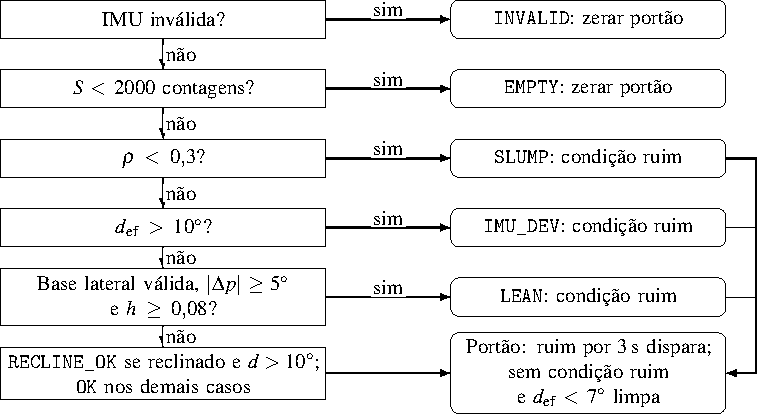
\includegraphics[width=364.59319pt,height=199.60779pt]{met-fusao.pdf}}
 \end{SingleSpace}
 \fonte{Elaborado pelos autores (2026)}
 \label{fig:met-fusao}
\end{figure}

\section{Painel}
\label{sec:met-painel}

O painel foi desenvolvido em Python e apresenta ao usuário a postura
identificada pelo colar, o contato dos sensores de força da cadeira, o tempo
de uso e a qualidade da postura ao longo do tempo, entre outras informações.
Ele recebe os dados da XIAO da cadeira pela conexão USB ou, sem fio, pelo
beacon BLE que essa placa transmite; neste caso, apenas escuta, sem
estabelecer conexão nem enviar comandos.

A função principal do painel é ajudar o usuário a encontrar a postura ideal:
com as amostras do colar em tempo real, ele indica quando, após o tempo de
espera, o usuário está em uma postura prejudicial, qual é essa postura e como
retornar à zona segura definida pela calibração.


    \renewcommand{\cleardoublepage}{}
    \renewcommand{\clearpage}{}
    
    \chapter{Testes e Resultados}\label{cap:resultados}

\section{Protocolos de teste}
\label{sec:res-protocolos}

Nove sessões com oito participantes registraram o sistema
com motor mudo. As posturas instruídas foram: (1) ereto, (2) curvado à
frente, (3) cabeça à frente com tronco apoiado, (4) escorregado,
(5--6) inclinado à esquerda/direita, (7) reclinado e (8--9) perna
esquerda sobre direita/direita sobre esquerda. Espera-se alerta em 2--6.
Mantiveram-se as posturas por cerca de 15\,s; aproveitaram-se 123 segmentos
e 50{,}74\,min com calibração válida, sem transições e os 2\,s iniciais.
Os rótulos são instruções do operador, sem medida anatômica independente.

Compararam-se as regras por reprodução temporal (\textit{replay}). No LOSO
(\textit{leave-one-subject-out}), ajustam-se os parâmetros com sete sujeitos
e avalia-se o omitido. A pontuação
balanceada é a média entre tempo alertado nos segmentos prejudiciais e
não alertado nos aceitáveis, incluindo pernas cruzadas, com igual peso por
segmento em cada grupo.Duas sessões em hardware usaram motor
ativo, com participante conhecido e sujeito novo.

\section{Caracterização em bancada}
\label{sec:res-bancada}

Nas quatro remontagens de bancada, a referência ereta variou cerca de
8\degree{} em \textit{pitch} e 21{,}6\degree{} em \textit{roll},
sustentando a calibração após vestir o colar. Nos FSRs, a histerese média
absoluta foi próxima de 52\,\% até 400\,g e 6\,\% a partir de 1\,kg.
Sob 1\,kg constante, a resistência caiu 7{,}4\,\% e 11{,}5\,\% em dois
sensores, em cerca de 11 e 12 minutos. A não linearidade, a histerese e o
\textit{creep} justificam medidas relativas à linha de base individual.

\section{Detecção nas capturas integradas}
\label{sec:res-deteccao}

A Figura~\ref{fig:res-dispersao} mostra a dispersão entre pessoas e
colocações no espaço absoluto, reduzida no ereto pela calibração.
Ainda assim, escorregado e reclinado se sobrepõem: suas médias
$(\Delta p,\Delta r)$ são $(-1{,}1;10{,}7)\degree{}$ e
$(-1{,}0;13{,}5)\degree{}$. A orientação isolada não informa o apoio do
quadril, o que motiva os FSRs.

\begin{figure}[H]
  \centering
  \caption{Dispersão angular nas capturas integradas: amostras estáveis
  e média $\pm1\sigma$ por postura, reunindo os oito participantes.}
  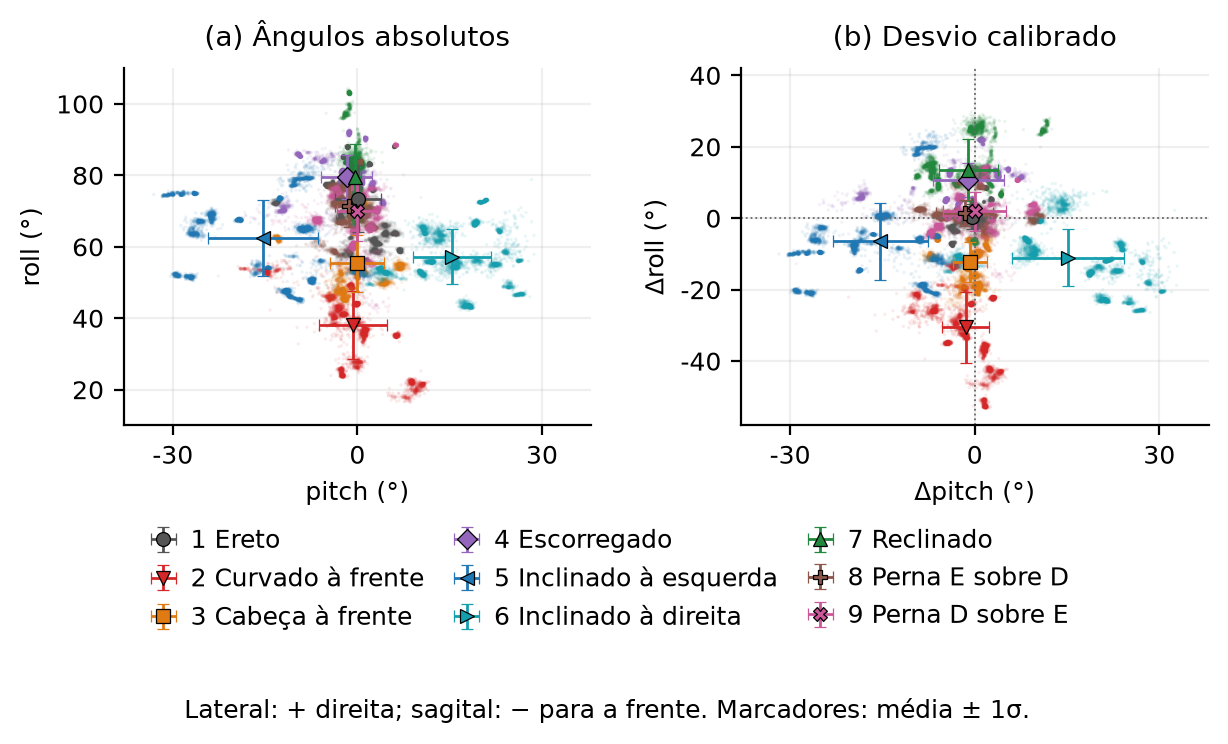
\includegraphics[width=\linewidth]{res_dispersao_posturas.png}
  \fonte[Fonte]{Elaborado pelos autores (2026)}
  \label{fig:res-dispersao}
\end{figure}

A Tabela~\ref{tab:res-comparacao} compara o mesmo recorte. A fusão final
foi ajustada com todos os dados; o LOSO avalia a transferência ao sujeito
omitido. A regra só-IMU não foi ajustada a essas capturas. Considera-se
detectado o segmento com ao menos um alerta, mesmo iniciado antes do
rótulo; por isso, informa-se também o tempo alertado.

\begin{table}[H]
  \centering
  \caption{Detecção por replay nas capturas de 21/10/2026.}
  \begingroup\SingleSpacing
  \small
  \begin{tabularx}{\linewidth}{@{}Xccc@{}}
    \toprule
    Indicador & Só-IMU & Fusão final & Fusão LOSO \\
    \midrule
    Segmentos prejudiciais detectados & 55/62 & 58/62 & 58/62 \\
    Tempo prejudicial com alerta (\%) & 84 & 93 & 92 \\
    Tempo ereto/reclinado com alerta (\%) & 29 & 2 & 3 \\
    Tempo de pernas cruzadas com alerta (\%) & 10 & 11 & 28 \\
    Pontuação balanceada por segmento & 0{,}834 & 0{,}935 & 0{,}901 \\
    \bottomrule
  \end{tabularx}
  \fonte[Fonte]{Elaborado pelos autores (2026)}
  \label{tab:res-comparacao}
  \endgroup
\end{table}

Na Figura~\ref{fig:res-alerta-sujeitos}, curvar à frente, escorregar e
inclinar à esquerda alertaram durante todo o recorte com a fusão final.
Cabeça à frente falhou em três de sete participantes: o movimento
localizado pouco alterou o IMU e preservou o contato. À direita de
Vinicius, desvio próximo ao limiar e carga oposta à esperada limitaram
o alerta a 38\,\% do tempo.

\begin{figure}[H]
  \centering
  \caption{Tempo com alerta por participante e postura: fusão final.}
  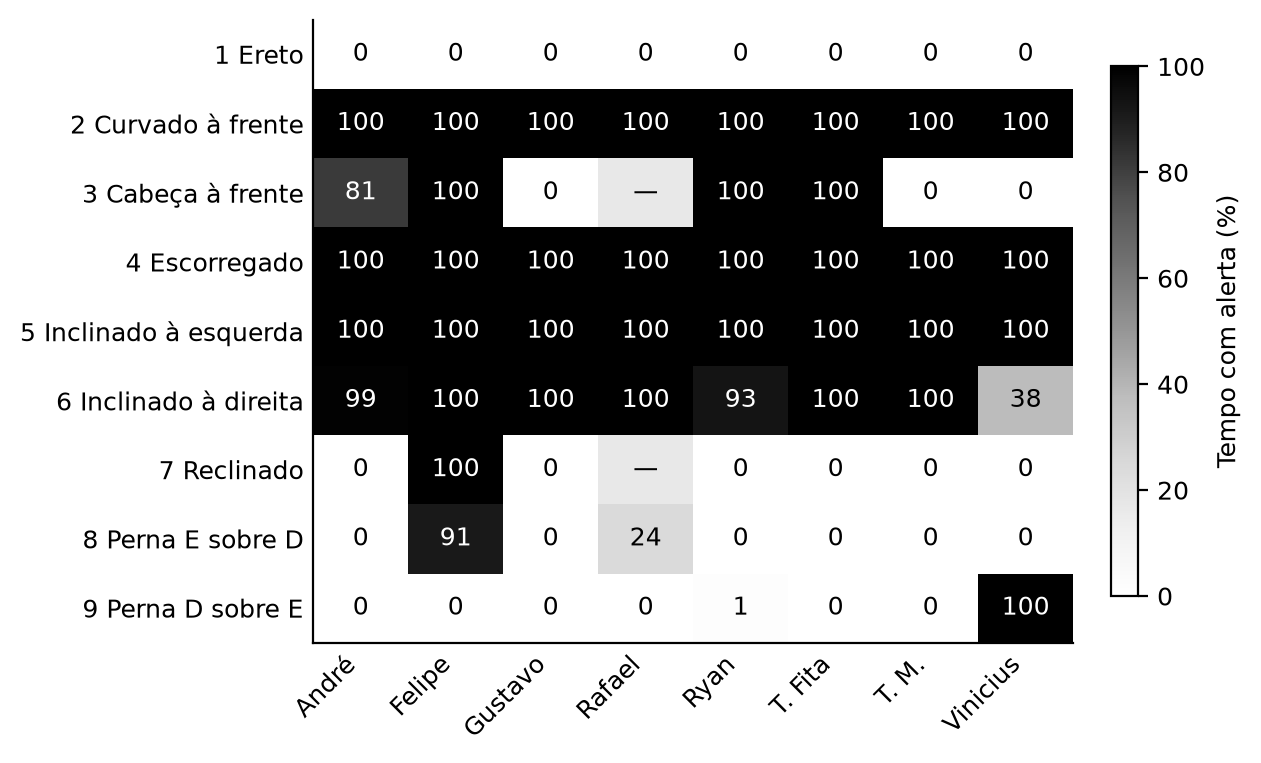
\includegraphics[width=\linewidth]{res_alerta_sujeitos.png}
  \fonte[Fonte]{Elaborado pelos autores (2026)}
  \label{fig:res-alerta-sujeitos}
  \begingroup\SingleSpacing
  {\footnotesize Espera-se alerta nas linhas 2--6 e ausência nas demais;
  células escuras indicam mais alerta, não necessariamente acerto. Traço:
  postura não registrada. E/D: esquerda/direita; T. Fita/T. M.: Thiago
  Fita/Thiago M.}
  \endgroup
\end{figure}

Em Felipe, desvio lateral próximo de 10\degree{} sem alteração no
assento foi compatível com deslocamento do colar e gerou falsos alarmes.
Vinicius escorregou ao cruzar as pernas: um alerta justificável foi contado
como falso pelo rótulo. Na ablação cumulativa, o maior ganho veio do
tratamento da reclinação apoiada; a confirmação lateral também acrescentou
falsos alarmes com pernas cruzadas.

\section{Validação em \textit{hardware}  e mostra}
\label{sec:res-hardware}

Na rodada guiada de André, participante do desenvolvimento, o alerta
nas placas ocupou 100\,\% do tempo estabilizado de 2--6 e 0\,\% das
demais posturas. Perceberam-se a vibração e sua interrupção ao retornar ao
ereto, verificando sensores, decisão e atuação.

Lucas, sujeito novo, realizou roteiro parcial: curvar à frente e escorregar
alertaram em 100\,\% do tempo estabilizado; inclinar à direita não
alertou. À esquerda, o alerta ocupou 9{,}2\,\%: a vibração perturbou o
IMU em cerca de $\pm10\degree{}$, interrompendo o alerta e reiniciando
os 3\,s. A correção reteve a última orientação sem motor durante a
vibração e elevou o alerta a 100\,\% no \textit{replay}, sem nova sessão controlada
em \textit{hardware} para confirmá-la.

Na mostra recolhida durante o evento Eureka, mais de 150 visitantes de biotipos
variados usaram o sistema com calibração individual e retorno vibratório;
a postura prejudicial foi detectada em praticamente todos os casos
observados, e os erros limitaram-se ao nome exibido para movimentos
combinados. Sem capturas rotuladas, essa evidência é qualitativa e não
integra os percentuais. O colar operou com uma célula de 600\,mAh durante
os dois dias (cerca de 20\,h) sem esgotá-la, o que indica corrente média
de no máximo cerca de 30\,mA; por extrapolação proporcional à capacidade
nominal, a célula de 1800\,mAh daria da ordem de 60\,h, valor não medido.

\section{Discussão}
\label{sec:res-discussao}

Com a fusão final, o alerta no reclinado caiu de 78\,\% para 5\,\%
do tempo; no escorregado, subiu de 72\,\% para 100\,\%. Em cerca de
176\,s de cadeira vazia, caiu de 71\,s para zero. O ganho decorre do
apoio e da presença medidos no assento; não se demonstrou contribuição
equivalente dos oito FSRs. Detectar o desvio é o objetivo; nomear posturas
mistas é complementar.

As capturas instruídas com oito participantes e um novo na validação
demonstram viabilidade, sem ensaio prolongado ou inferência populacional.
Persistem falhas com cabeça à frente, deslocamento do colar e posturas
mistas. Não alertar por pernas cruzadas é opção de escopo, sem conclusão
clínica. Não se mediram corrente e latência em bancada nem efeitos
duradouros sobre hábitos ou distúrbios musculoesqueléticos.


    \renewcommand{\cleardoublepage}{}
    \renewcommand{\clearpage}{}
    
    \chapter{Conclusões e Trabalhos Futuros}\label{cap:conclusao}

Este trabalho desenvolveu um sistema embarcado e autônomo que detecta posturas
sentadas prejudiciais e alerta o usuário por vibração, fundindo na cadeira a
distribuição do peso e a orientação da parte superior das costas medida pelo
colar, sem computador, aplicativo ou nuvem.

Quanto aos objetivos específicos, a variação da referência de postura ereta
entre pessoas e entre colocações do sensor mostrou-se da mesma ordem do desvio
a detectar, o que tornou a calibração individual por botão uma condição de
funcionamento. O colar e a cadeira foram construídos, alimentados por
bateria e integrados por um enlace sem perda de pacotes nos ensaios. O
alerta por vibração foi percebido pelos usuários e cessou com a correção da
postura. Com oito participantes, deixando cada um fora do ajuste dos
parâmetros, o sistema alertou em 94\,\% de postura prejudicial,
com alerta em 3\,\% do tempo em postura ereta ou reclinada; com pernas
cruzadas, que a regra não pretende sinalizar, essa fração chegou a 28\,\%. A principal contribuição é a fusão: os sensores da cadeira,
inadequados como medidores de força, bastaram como indicadores de contato para
não alertar ao reclinar com o quadril apoiado ou ao levantar-se e para
detectar o escorregamento do quadril.

Os resultados indicam a viabilidade técnica da abordagem: os participantes
das capturas tinham biotipos variados, mais de 150 visitantes da mostra
Eureka usaram o protótipo com detecção consistente, e uma célula de
600\,mAh sustentou o colar pelas cerca de 20\,h da mostra. Os percentuais,
porém, vêm de posturas instruídas, e não se avaliou efeito sobre a saúde.
Permanecem como limitações a projeção isolada da cabeça, as pernas
cruzadas, a fixação do colar e a interação entre a vibração e o sensor.

Como trabalhos futuros, propõem-se validar o sistema com mais participantes,
posturas naturais e uso prolongado, já com a correção da interferência do
motor embarcada; adotar vibração com pausas, menos incômoda; compensar a
deriva lenta da referência e aprimorar a fixação do colar; tratar a projeção
da cabeça com outra posição do sensor ou um segundo sensor; e estudar a
mudança de hábito e os sintomas osteomusculares em uso longitudinal.



\endgroup

% ----------------------------------------------------------
% ELEMENTOS PÓS-TEXTUAIS (Referências, Glossário, Apêndices)
% ----------------------------------------------------------
%\postextual

% Referências bibliográficas
\selectlanguage{brazil}
\bibliography{bibliografia}

\end{document}
